\section{Parametrisierte Algorithmen}

\begin{takeaway}
    \item Parametrisierter Algorithmus, fpt
    \item Standard-Parametrisierung
    \item Kernbildung
    \item (Sichere) Datenreduktionsregel
    \item Kronenzerlegung
    \item Tiefenbeschränkte Suchbäume
    \item Iterative Kompression
    \item Baumzerlegung, Baumweite; bramble, bramble number
    \item Probleme: Edge Clique Cover, Cluster Editing, Steinerbaum
\end{takeaway}

\paragraph{Idee}
Verallgemeinerung von pseudopolynomiellen Algorithmen:
Laufzeit hängt von der Eingabegrösse nur polynomiell ab, aber darf extrem gross werden in der Grösse eines Parameters.
Partitionierung in Problemklassen entlang des Parameters.

\paragraph{Parametrisierung}
Sei $U$ ein Entscheidungsproblem, $L$ die Sprache der Eingaben.
$\Par: L \mapsto \N$ ist eine \emph{Parametrisierung} von $U$ falls gilt:
\begin{enumerate}[label=(\roman*)]
    \item $\Par$ ist in Polynomzeit berechenbar
    \item Für unendlich viele $k \in \N$ ist die Parameter-$k$-Menge für $U$
    $$ Set_U(k) := \{ I \in L \st \Par(I) = k \} $$ unendlich.
    Dies stellt sich dass $\Par$ nichttrivial ist, z.B. nicht etwa $\Par(I) = |I|$.
    In anderen Worten, für jeden Parameterwert soll es beliebig viele Probleminstanzen geben.
\end{enumerate}
Ein Algorithmus $\A$ heisst \emph{$\Par$-paremetrisierter Polynomzeit-Algorithmus} für $U$ falls gilt:
\begin{enumerate}[label=(\roman*)]
    \item $\A$ löst $U$
    \item $ \exists \text{ Polynom } p \; \exists \text{ (berechenbare) Funktion } f : \N \mapsto \N$
    so dass $\forall I \in L$:
    $$\Time_\A(I) \leq f \big( \Par(I) \big) \cdot p(|I|) $$
\end{enumerate}
Dann heisst $U$ \emph{fixed-parameter-tractable bezüglich $\Par$}.
$\A$ heisst auch \emph{fpt-Algorithmus für $U$ bezüglich $\Par$} und läuft in fpt-Zeit.

\underline{Beispiel:}
Sei $U$ ein Zahlproblem und sei $Val(I) := \max \{ |x_i| \}$.
Es gilt $Max-Int(I) \leq 2^{Val(I)}$ und ist $Val$ eine Parametrisierung von $U$.

\paragraph{Ansätze}
Die \emph{Standard-Parametrisierung} wählt als Parameter die Grösse der gewünschten Lösung (z.B. Grösse des VCs).
Die \emph{Strukturelle Parametrisierung} wählt eine bestimmte Eigenschaft der Eingabe (z.B. maximaler Knotengrad).
Andere Ansätze betrachten wir im Folgenden.


\subsection{Kernbildung}

\paragraph{Idee}
Polynomielles Preprocessing, Datenreduktion, um die Instanz auf einen \emph{Kern} zu verkleinern,
der in seiner Grösse nur noch vom Parameter abhängt.
Diesen Kern dann mit bekannten Algorithmen (oder brute force) lösen.

\paragraph{Kernbildung (kernelisation)}
Sei $(U, \Par)$ ein parametrisiertes Entscheidungsproblem, $L$ die Sprache der JA-Instanzen von $U$.
Ein \emph{Kernbildungs-Algorithmus} für $(U, \Par)$ ist ein Polynomzeit-Algorithmus $\A$ der jede Eingabe $(I, k)$
in eine neue Eingabe $(I', k')$ (den \emph{Kern (kernel)}) transformiert so dass:
\begin{enumerate}[label=(\roman*)]
    \item $ I \in L \iff I' \in L $ (Korrektheit)
    \item $ |I'| + k' \leq g(k) $ für $g : \N \mapsto \N$ (neue Grösse nur abhängig vom alten Parameterwert $k$)
\end{enumerate}

Eine \emph{Reduktionsregel} von $\A$ heisst \emph{sicher}, wenn sie (i) erfüllt.

\paragraph{Beispiel: VCP} \mbox{} \\
\underline{Reduktionsregel:}
Sei $S \subseteq V$ ein VC von $G$ so dass $|S| \leq k$. Dann enthält $S$ alle Knoten mit $\deg_G(v) > k$ (warum?).
Dann gilt für ein solches $v$:
$$ (G, k) \in VCP \iff (G-\{v\}, k-1) \in VCP $$
Zusätzlich entferne alle isolierten Knoten mit $\deg_G(v) = 0$ (sie decken keine Kanten ab).

Zu zeigen: wenn die Regel nicht mehr anwendbar ist, dann hat der verbleibende Graph $G'$ entweder kein vertex cover,
oder aber er ist ``klein genug'' (nur noch anhängig von $k$), also ein Kern.

\underline{Beobachtung:}
Sei $G$ ein Graph ohne isolierten Knoten, mit einem vertex cover der Grösse $m$ und mit $\max \deg_G(v) \leq k$.
Dann gilt $|V| \leq m \cdot (k+1)$ (warum?).%
\footnote{Falls $|V| > k \cdot (k+1)$, dann wir wissen dass $ I \notin L$ und können NEIN ausgeben.}

\underline{Theorem:}
Diese Reduktionsregeln berechnen einen Kern der Grösse $\bigO (k^2)$ in Zeit%
\footnote{Unter der Annahme dass die Knotengrade bereits gegeben sind, ansonsten $\bigO (k \cdot n + m)$.}
$\bigO (k \cdot n)$.

\underline{Parametrisierter Algorithmus:}
Berechne einen Kern $(G', k')$. Wenn der Kern zu gross ist, geben NEIN aus.
Andernfalls prüfe durch vollständige Suche ob ein VC mit $|S'| \leq k'$ existiert.

\underline{Theorem:}
Dies ist ein fpt-Algorithmus bzgl. der Standard-Parametrisierung. Die Laufzeit beträgt
$\bigO (k \cdot n + k^{2k+2}) \subseteq \bigO (k^{2k+2} \cdot n)$.

\paragraph{Theorem}
Sei $(U, \Par)$ ein parametrisiertes Entscheidungsproblem. \\
Ein fpt-Algorithmus für $(U, \Par)$ existiert $\iff$ Ein Kernbildungsalgorithmus für $(U, \Par)$ existiert.

\paragraph{Edge Clique Cover Problem ECCP} \mbox{} \\
Eingabe: ungerichteter Graph $G=(V,E)$, $k \leq \N$ \\
Ausgabe: JA falls $k$ Cliquen\footnote{Clique: Knotenmenge so dass alle Knoten paarweise miteinander verbunden sind,
d.h. einen vollständigen Teilgraphen bilden.}
$C_1, \dots, C_k$ existieren, so dass $E = \bigcup_{i=1}^k E(C_i)$ (jede Kante ist in mind. einer Clique), sonst NEIN.

\underline{Reduktionsregeln:}
\begin{enumerate}[label=(\roman*)]
    \item $(G, k) \xrightarrow{\text{isolierter Knoten } u} (G-\{ u \}, k)$
    \item $(G, k) \xrightarrow{\text{isolierte Kante } e=\{u,v\} } (G-\{ u,v \}, k-1)$
    \item $(G, k) \xrightarrow{\{u,v\} \in E \text{ s.t. } \{u,v\} \subsetneq N[u] = N[v] } (G-\{ u \}, k)$ \\
    $N[u]$ ist die \emph{geschlossene Nachbarschaft} von $u$, also alle benachbarten Knoten und $u$ selbst.
\end{enumerate}

\underline{Theorem:} Das ECCP hat einen Kern mit $\leq 2^k$ Knoten.


\subsubsection{Kronenzerlegung}

Ziel: statt einem quadratischen Kern suchen wir einen linearen Kern für das VCP. \\
Bisher genutzte Strukturen zur Reduktion: hoher Knotengrad, gleiche geschlossene Nachbarschaft.

\paragraph{Kronenzerlegung (crown decomposition)}
Die \emph{Kronenzerlegung} von $G=(V,E)$ ist eine Partitionierung $V = C \cup H \cup B$ so dass:
\begin{enumerate}[label=(\roman*)]
    \item $C \neq \emptyset$ ist ein independent set\footnote{Eine Menge von Knoten zwischen denen es keine Kante gibt.} in $G$
    \item $N(C) = H$ (keine Kanten zwischen $C$ und $B$)
    \item Die Kanten zwischen $C$ und $H$ enthalten ein Matching $M$ mit $|M| = |H|$ ($M$ \emph{saturiert} $H$).
\end{enumerate}

\begin{figure}[h]
    \centering
    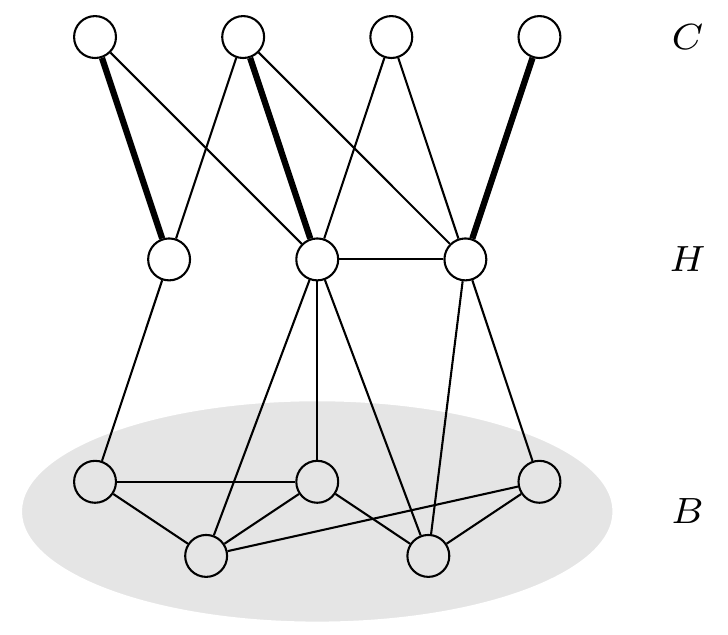
\includegraphics[scale=0.3]{images/crown-decomp.png}
    \caption{Kronenzerlegung: crown, head, body (Quelle: Vorlesung)}
    \label{fig:crown-decomp}
\end{figure}

\paragraph{Satz von König}
Sei $G$ ein ungerichteter bipartiter Graph, sei $M$ ein Matching maximaler Kardinalität,
sei $S$ ein vertex cover minimaler Kardinalität.
Dann gilt $|M| = |S|$.

\underline{Theorem:} $M$ und $S$ können in Polynomzeit berechnet werden.

\paragraph{Lemma}
Sei $G$ ungerichtet, ohne isolierte Knoten, mit $|V| \geq 3k+1$.
Dann existiert ein Polynomzeitalgorithmus der
\begin{enumerate}[label=(\roman*)]
    \item entweder eine Kronenzerlegung berechnet
    \item oder ein Matching $M$ mit $|M| \geq k+1$ findet.
\end{enumerate}
Beweis siehe Buch, Kapitel 6.2, Seite 145f.

\paragraph{Reduktion für VCP} \mbox{} \\
\underline{Lemma:}
Sei $G$ ein Graph mit Kronenzerlegung $V = C \cup H \cup B$ und sei $k \in \N$. Dann gilt: \\
$$ (G, k) \in VCP \iff \Big( G - (C \cup H), k - |H| \Big) \in VCP $$

\underline{Theorem:} Ein Kernbildungsalgorithmus mit obiger Reduktionsregel findet einen Kern mit $\leq 3k$ Knoten.


\subsection{Tiefenbeschränkte Suchbäume}

\paragraph{Idee}
Vollständige Suche über alle möglichen Lösungen, aber mit Suchbaumtiefe beschränkt im Parameter.

\paragraph{Beispiel: VCP}
Beobachtung: in jedem vertex cover $S$ gilt $\forall e = \{v_1, v_2\} : v_1 \in S \vee v_2 \in S$.
Daher verzweige von $(G, k)$ nach $(G-\{v_1\}, k-1)$ und $(G-\{v_2\}, k-1)$.
In den Blättern $(G_j, 1)$ ist das VCP trivial.
Dieser Suchbaum hat Tiefe $k$ und $2^{k-1}$ Blätter.
Gesamtlaufzeit: $\bigO (2^k \cdot n)$.

\paragraph{Cluster Editing Problem CEP} \mbox{} \\
Eingabe: Graph $G = (V, E)$, $k \in \N$ \\
Ausgabe: JA falls durch Löschen/Einfügen von $\leq k$ Kanten $G$ in eine Vereinigung (union) von disjunkten Cliquen
(= jeder connected component ist eine Clique) transformiert werden kann, sonst NEIN. \\
Bekannterweise NP-schwer.

\underline{Theorem:}
Graph $G$ besteht aus disjunkten Cliquen \\
$\iff$ $G$ enthält \emph{keinen} Pfad aus drei Knoten\footnote{In eine Clique bilden drei Knoten einen Kreis, keinen Pfad.}\\
$\iff$ es gibt \emph{keine} paarweise verschiedenen $u, v, w \in V : \{u,v\}, \{v,w\} \in E \wedge \{u,w\} \notin E$

\begin{figure}[h]
    \centering
    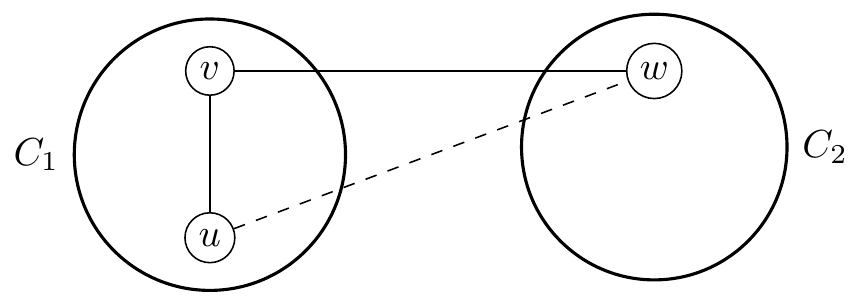
\includegraphics[scale=0.35]{images/cluster-editing.png}
    \caption{Cluster Editing Situation (Quelle: Vorlesung)}
    \label{fig:cluster-editing}
\end{figure}

\underline{Algorithmus:}
Teste ob $G$ bereits eine Vereinigung disjunkter Cliquen ist, oder ob $k=0$.
Wenn nicht, finde $u,v,w \in V$ mit obiger Bedingung.
Rekursiere auf
$G_1 = \big(V, E   -  \{ \{u,v\} \} \big)$,
$G_2 = \big(V, E   -  \{ \{v,w\} \} \big)$,
$G_3 = \big(V, E \cup \{ \{u,w\} \} \big)$.
Laufzeit\footnote{Die Rekursionsformel $T(k) = 3 \cdot T(k-1)$ gibt $\bigO (3^k)$ rekursive Aufrufe.}:
$\bigO (n^3 \cdot 3^k)$.


\subsection{Iterative Kompression}

\paragraph{Idee}
Gegeben ein Kompressionsalgorithmus der aus einer (bzgl. dem Schwellwert) etwas zu grossen Lösung eine kleinere,
gültige Lösung in fpt-Zeit berechnet.
Iteriere: Instanz vergrössern, komprimieren, usw.:
\\
\begin{align*}
(I_0, k_0) & \text{ mit Lösung } S_0^*, |S_0^*| \leq k_0 \\
\xrightarrow{\text{Instanz vergrössern}}
(I_1, k_1) & \text{ mit Lösung } S_1,   |S_1|   > k_1 \\
\xrightarrow{\text{komprimieren}}
(I_1, k_1) & \text{ mit Lösung } S_1^*, |S_1^*| \leq k_1 \\
& \dots
\end{align*}

\paragraph{Disjoint Vertex Cover Problem DVCP} \mbox{} \\
Eingabe: $G=(V,E)$, vertex cover $W$, $k \in \N$ \\
Ausgabe: JA falls es ein vertex cover $S$ gibt mit $|S| \leq k \wedge S \cap W = \emptyset$ sonst NEIN.

\underline{Lemma:}
Jede DVCP-Instanz $(G, W, k)$ kann in Zeit $\bigO (|V|^2)$ gelöst werden (warum?\footnote{
Es reicht zu prüfen ob $N(W)$ ein vertex cover ist}).

\paragraph{Beispiel: VCP}
Idee: füge einen Knoten nach dem anderen hinzu.
Starte mit $S_1^* = \emptyset$. In jeder Iteration setzte $S_i \leftarrow S_{i-1}^* \cup \{v_i\}$ und benutze
$\A_{compress}(G_i, S_i, k)$ um entweder $S_i^*$ zu finden oder NEIN.
Details siehe Buch, Algorithmen 6.6+6.7, Seite 151ff.

\underline{Kompression:} Idee: probiere alle möglichen intersections $X$ des gesuchten VCs mit $S$ aus: \\
If $|S| \leq k$ return $S$.
For all $X \subseteq S$ with $|X| \leq k$ do:
solve DVCP on $(G-X, S-X, k-|X|)$
-- if YES return $X \cup N(S-X)$.
\\
Laufzeit: $\bigO (2^k \cdot n^2)$ also gesamt: $\bigO (2^k \cdot n^3)$.


\subsection{Dynamische Programmierung für den Steinerbaum}

\paragraph{Steinerbaum-Problem STP} \mbox{} \\
Eingabe: $G=(V,E)$ mit Kantenkosten $c : E \mapsto \N$, \emph{Terminalen} $S \subseteq V$,
\emph{Nicht-Terminale/Steiner-Knoten} $N = V-S$ \\
Lösungen: Teilbaum $T$ von $G$ (\emph{``Steinerbaum''}) der alle Knoten aus $S$ enthält (und einige aus $N$) \\
Kosten: $cost(T, (G,c,S)) = c(T) = \sum_{e\in E(T)} c(e) = $ Summe der Kanten = ``Grösse'' des Baums \\
Ziel: $\min$

\paragraph{DP-Ansatz}
Annahme: alle Blätter sind Terminale (warum?).

Beobachtung: falls $Y \subseteq N$ gegeben ist dann ist das STP einfach: berechne MST von $S \cup Y$. \\
$\implies$ k-parametrisierter Algorithmus mit $k = |N|$.

Uninteressant, wir schauen im Folgenden ein DP mit dem Parameter $k = |S|$ an.
Für alle $X \subseteq S$ und alle $v \in V-X$ berechne zwei Steinerbäume:
\begin{enumerate}
    \item Auf Instanz $(G, c, X)$ einen Steinerbaum mit minimalen Kosten $g(X)$.
    \item Auf Instanz $(G, c, X \cup \{v\})$ einen Steinerbaum mit minimalen Kosten $g_{in}(X, v)$ so dass $v$ ein innerer Knoten ist (d.h. $\deg(v) \geq 2$).
\end{enumerate}

\paragraph{Lemma}
Es gilt:
\begin{equation}
g_{in}(X, v) = \min_{\emptyset \neq X' \subset X} \left\{
    g(X' \cup \{v\}) + g \left( (X-X') \cup \{v\} \right)
\right\}
\end{equation}
\begin{equation}
g(X \cup \{v\}) = \min \left\{
    \min_{w \in X} \left\{ p(v,w) + g(X) \right\},
    \min_{w \in V-X} \left\{ p(v,w) + g_{in}(X,w) \right\}
\right\}
\end{equation}
wobei $p(v,w)$ die minimalen Kosten eines Pfades von $v$ nach $w$ in $G$ sind.
Beweis siehe Buch Kapitel 6.5, Seite 159ff.

\paragraph{Dreyfus-Wagner Algorithmus}
Eingabe $(G, c, S)$.
Berechne $p(v, w)$ für alle $v,w \in V$.
Initialisiere $g(\{x,y\}) := p(x,y)$ für alle $x,y \in S$.
Für alle $X \subseteq S$ mit $|X| \in [2, |S|-1]$ und alle $v \in V-X$ berechne $g_{in}(X, v)$ und $g(X \cup \{v\})$.
Gebe $g(S)$ aus.
\\
Laufzeit: $\bigO (n^2 \log n + n \cdot m + (k^2 + )\; 3^k \cdot n + 2^k \cdot n^2)$


\subsection{Baumzerlegung}

\paragraph{Motivation}
Viele schwere Graphprobleme sind auf Bäumen einfach.
Z.B. im VCP Reduktionsregel durch Entfernen von Blättern und ihren Nachbarn, und Hinzufügen der Nachbarn ins VC.
\\
Ziel: ``Baumähnlichkeit'' von Graphen beschreiben.

\paragraph{Definition (Baumzerlegung)}
Eine \emph{Baumzerlegung (tree decomposition)} von $G$ ist ein Paar $D = (T, B)$
wobei $T = (V_T, E_T)$ ein Baum ist.
Sei $I$ eine Indexmenge, die die Knoten aus $V_T$ aufzählt.%
\footnote{Dies erlaubt es uns getrennt über die Knotenmenge $V_T$ des Baums $T$ und über die bags zu sprechen.}
Sei $B$ eine Label-Funktion $B : I \mapsto 2^V$ die jedem Index $i$ von $V_T$ eine Knotenmenge $X_i \subseteq V$
(einen \emph{bag}) zuordnet, so dass:
\begin{enumerate}[label=(\roman*)]
    \item $ \bigcup_{i \in I} X_i = V $ (alle Knoten kommen vor)
    \item $ \forall \{u,v\} \in E \; \exists i \in I : u, v \in X_i $ (alle Kanten in einem bag)
    \item $ \forall v \in V $ bilden die bags $X_i$ mit $v \in X_i$ einen Teilbaum von $T$ (Zusammenhang, Lokalität)
\end{enumerate}

Die \emph{Weite} von $D$ ist $\max \{|X_i|\} - 1$.\footnote{Das $-1$ ist kosmetisch damit echte Bäume eine Baumweite von 1 haben.} \\
Die \emph{Baumweite} $\tw(G)$ von $G$ ist die minimale Weite über alle möglichen Baumzerlegungen.

\begin{figure}[h]
    \centering
    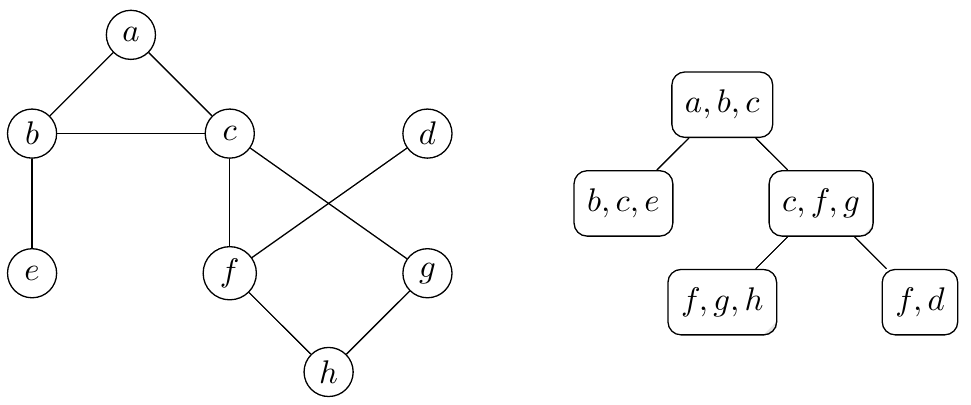
\includegraphics[scale=0.4]{images/tree-decomp.png}
    \caption{Graph $G$ (links) und seine Baumzerlegung $D$ (rechts) (Quelle: Vorlesung)}
    \label{fig:tree-decomp}
\end{figure}

\paragraph{Beobachtungen}
\begin{itemize}
    \item Sei $G$ ein Baum. Dann ist $\tw(G) = 1$.
    \item Sei $G$ ein Kreis. Dann ist $\tw(G) = 2$.
    \item Sei $G$ ein Graph, $v \in V, e \in E$.
    Dann ist jede Baumzerlegung $D$ für $G$ auch eine Baumzerlegung für $G-e$.
    Auch kann $D$ in eine Baumzerlegung $D'$ für $G-v$ transformiert werden mit gleicher oder kleinerer Weite
    (z.B. durch Entfernen von $v$ aus $D$).
    \\
    $\implies$ Die Baumweite ist monoton: zusätzliche Knoten/Kanten verringern nicht die Baumweite.
    \item Sei $G$ ein Graph, sei $C \subseteq V$ eine Clique der Grösse $|C| = k$.
    Dann gilt $\tw(G) \geq k-1$ (und es existiert ein bag, der alle Knoten der Clique enthält).
    \\
    $\implies$ grosse Cliquen $\Rightarrow$ grosse Baumweite.
    ABER kleine Cliquen $\nRightarrow$ kleine Baumweite (z.B. $l \times l$-Gitter-Graph).
    \\
    $\implies$ Konzept der Clique kein genügendes Modell für den Zusammenhang
    (und damit der Baumähnlichkeit) eines Graphen.
    Verallgemeinerung: statt Knoten die sich gegenseitig berühren betrachten wir
    \underline{Mengen von} Knoten die sich gegenseitig berühren.
\end{itemize}

\paragraph{Definition (bramble)}
Sei $G$ ein Graph, sei $\B = \{B_1, \dots, B_k\}$ mit $B_i \subseteq V$
Wir sagen dass $B_i, B_j$ sich \emph{berühren (touch)}, falls
$B_i \cap B_j \neq \emptyset$ oder $\exists \{x_i, x_j\} \in E : x_i \in B_i \wedge x_j \in B_j$.
\\
Wenn alle $B_i$ sich paarweise berühren, dann heisst $\B$ \emph{bramble} (``Dornen-/Brombeergestrüpp'') von $G$.

$C \subseteq V$ heisst \emph{Überdeckung (cover)} von $\B$, falls $C \cap B_i \neq \emptyset$ für alle $i$.
\\
Die \emph{Ordnung (order)} von $\B$ ist die Grösse einer minimalen Überdeckung von $\B$.
\\
Die \emph{bramble number} $\bn(G)$ von $G$ ist die maximale Ordnung eines bramble von $G$.

\underline{Beispiel:}
In einem $k \times k$-Gitter-Graph sei ein ``Kreuz'' $C_{i,j}$ die Vereinigung von Reihe $i$ und Spalte $j$.
Dann ist $\B = \{C_{i,j}\}$ ein bramble von $G$ der Ordnung $k$ und jeder Reihe und jede Spalte ist
eine Überdeckung von $\B$.

\paragraph{Theoreme}
\begin{itemize}
    \item Sei $G$ ein Graph. Dann gilt $\bn(G) = \tw(G) + 1$. \\
    $\longrightarrow$ Die bramble number beschreibt die Grösse eines grössten bags in einer optimalen Baumzerlegung.
    \item Die Bestimmung der Baumweite eines Graphen ist NP-schwer.
    (?Ebenso die Konstruktion einer beliebigen Baumzerlegung?) \\
    $\longrightarrow$ Problem: das Parameter eines parametrisierten Algorithmus' sollte in Polynomzeit berechenbar sein!
    \item Sei $G$ ein Graph mit $\tw(G)=k$. Dann kann man eine Baumzerlegung der Grösse/Weite $\leq 5k$
    in Zeit $2^{\bigO(k)} \cdot n$ berechnen.
\end{itemize}



